\documentclass[xcolor=pdftex,dvipsnames,table,mathserif,aspectratio=169]{beamer}
\usetheme{metropolis}

%\usetheme{Darmstadt}
%\usepackage{times}
%\usefonttheme{structurebold}

\usepackage[english]{babel}
%\usepackage[table]{xcolor}
\usepackage{pgf,pgfarrows,pgfnodes,pgfautomata,pgfheaps}
\usepackage{amsmath,amssymb,setspace,centernot}
\usepackage[latin1]{inputenc}
\usepackage[T1]{fontenc}
\usepackage{relsize}
\usepackage{stmaryrd}
\usepackage{pdfpages}
\usepackage{booktabs}
\usepackage[absolute,overlay]{textpos} 


\newenvironment{reference}[2]{% 
  \begin{textblock*}{\textwidth}(#1,#2) 
      \footnotesize\it\bgroup\color{red!50!black}}{\egroup\end{textblock*}} 

\DeclareMathSizes{10}{10}{6}{6} 
\AtBeginSection[]{
  \begin{frame}
  \vfill
  \centering
  \begin{beamercolorbox}[sep=8pt,center,shadow=true,rounded=true]{title}
    \usebeamerfont{title}\insertsectionhead\par%
  \end{beamercolorbox}
  \vfill
  \end{frame}
}
\begin{document}
\title{Lecture 5: Pricing Equilibria and Mergers}
\author{Chris Conlon}
\institute{Grad IO}
\date{\today}

\frame{\titlepage}

\section{Antitrust and Mergers}

\begin{frame}
\frametitle{What is Antitrust?}
 \begin{itemize}
\item Current Debate: should we maximize \alert{efficiency/social surplus} or should we focus on \alert{consumer surplus}.
\begin{itemize}
\item US antitrust law focuses primarily on harm to consumers.
\item EC tends to also worry about harm to competing firms.
 \end{itemize}
 \item We know about DWL from market power from undergrad economics. However, without profits, why would firms innovate or perform R\&D?
 \begin{itemize}
\item Law understands this and awards temporarily monopolies via patents.
 \end{itemize}
\item Today, I am going to focus mostly on \alert{horizontal mergers} among competitors.
\begin{itemize}
\item Most of this is known as \alert{unilateral effects} (which is a terrible name).
\item Also worry about \alert{coordinated effects} which mean the nature of equilibrium changes.
 \end{itemize}
 \end{itemize}
\end{frame}

\begin{frame}
\frametitle{Antitrust Legislation : Sherman Act (1890)}
 \begin{description}
\item [Section 1]``Every contract, combination in the form of trust or otherwise, or conspiracy, in restraint of trade or commerce among the several States, or with foreign nations, is declared to be illegal'' (Violation involves an \alert{agreement}).
\item [Section 2] ``Every person who shall monopolize, or attempt to monopolize, or combine or conspire with any other person or persons, to monopolize any part of the trade or commerce among the several States, or with foreign nations, shall be deemed guilty of a felony''.
 \end{description}
 Three \textit{per se} violations
 \begin{itemize}
 \item (1) price fixing (2) horizontal market division (3) refusals to deal.
 \item Other violations are \textit{rule of reason}.
 \end{itemize}
 
\end{frame}

\begin{frame}
\frametitle{Antitrust Legislation : Clayton Act (1914)}
 \begin{description}
\item [Section 2] Prohibits some forms of price discrimination, but only when it lessens competition.
\item [Section 3] Prohibits sales based on the condition that the buyer not buy from your competitor (includes tying and exclusive dealing), but only when effect may be to substantially lessen competition.
\item [Section 7] Prohibits mergers where the effect of such acquisition may be substantially to lessen competition, or tend to create a monopoly in any line of commerce.
\item [Section 8] Prevents a person from being a director of multiple competing firms.
 \end{description}
\end{frame}

\begin{frame}
\frametitle{Antitrust Legislation : Hart-Scott-Rodino Act (1976)}
 \begin{itemize}
\item Required pre-notification and registration of large mergers
\begin{itemize}
\item Transaction: \$78.2 million
\item Size of Person: \$156.3 M with target of \$15.6 M or total transaction of \$312.6M
\item These are ``inflation adjusted'' each year.
\end{itemize}
\item Initial review period is 30 days after which DOJ/FTC can request additional information or allow merger to proceed.
\item Second review usually involves detailed information about  price-cost margins, market shares, etc. (Usually more info available than to academic researchers).
\item Can request information company would reasonably have (customer surveys, etc.).
\item After second review can ask for \alert{injunctive relief} or \alert{remedies} which merging parties can oppose in court.
 \end{itemize}
\end{frame}

\begin{frame}
\frametitle{DOJ/FTC Horizontal Merger Guidelines}
 \begin{itemize}
\item DOJ/FTC describe markets as:
\begin{itemize}
\item Highly Concentrated: $HHI \geq 2500$.
\item Moderately Concentrated: $HHI \in [1500,2500]$. $\Delta HHI \geq 250$ merits scrutiny.
\item Un-Concentrated: $HHI \leq 1500$.
\end{itemize}
\item Also consider \alert{unilateral effects}/UPP and \alert{coordinated effects}.
\item Three steps:
\begin{enumerate}
\item Market Definition
\item Measure Concentration/Initial Screening
\item Merger Simulation
\end{enumerate}
 \end{itemize}
\end{frame}

\begin{frame}
\frametitle{Step 1: Market Definition}
SSNIP
 \begin{itemize}
\item Small but significant and non-transitory increase in price (SSNIP): smallest relevant market where a hypothetical monopolist could impose a 5\% price increase. (For at least one year).
\item Under linear demand this amounts to a price cost margin and an elasticity (sometimes the \alert{critical elasticity}).
 \end{itemize}
 Tricky Examples:
  \begin{itemize}
\item Whole Foods vs. Wild Oats
\item Cellophane Fallacy.
 \end{itemize}
\end{frame}

\begin{frame}
\frametitle{Step 2: Concentration/Screening}
 \begin{itemize}
\item After we define the relevant market, compute the relevant HHI or UPP.
\item There can be both geographic and product market issues in the relevant market.
\item Some markets may be highly concentrated and others may not be.
\item Can ask for \alert{divestitures} as part of a \alert{remedy} if there are a few problematic markets in an otherwise uncontroversial merger.
 \end{itemize}
\end{frame}


\begin{frame}
\frametitle{Step 3: Merger Simulation}
 \begin{itemize}
\item Simulate the price effects of the merger
\item Take into account likely cost synergies (sometimes there are none).
\item Estimate post-merger prices and welfare.
 \end{itemize}
 This is what we will talk about next.
\end{frame}

\section{Merger Simulation}

\begin{frame}
\frametitle{Merger Simulation: Two Options}
 \begin{itemize}
\item Partial Merger Simulation
 \begin{itemize}
\item Simulate a new price for $p_j$ after acquiring good $k$ holding the prices of all other goods $(p_k,p_{-j})$ fixed.
\item Repeat for $p_k$ and all other products involved in the merger.
\item Compare price increases to \alert{synergies} or cost savings.
 \end{itemize}
 \item Full Merger Simulation
 \begin{itemize}
\item Write down the full system of post-merger FOC.
\item Adjust post-merger marginal costs for potential synergies.
\item Solve for all prices at the new (post-merger) equilibrium $(p_j,p_k,p_{-j})$.
 \end{itemize}
 \end{itemize}
\end{frame}

\begin{frame}
\frametitle{Differentiated Products Bertrand}
Recall the multi-product Bertrand FOCs:
\begin{eqnarray*}
\arg \max_{p \in \mathcal{J}_f} \pi_f (\mathbf{p}) &=& \sum_{j \in \mathcal{J}_f} (p_j - c_j) \cdot q_j(\mathbf{p}) \\
\rightarrow 0&=& q_j(\mathbf{p}) + \sum_{k \in \mathcal{J}_f} (p_k - c_k) \frac{\partial q_{k}}{\partial p_j}(\mathbf{p})
\end{eqnarray*}
It is helpful to define the matrix $\Omega$ with entries:
\begin{eqnarray*}
\Omega_{(j,k)}(\mathbf{p}) = \left\{\begin{array}{lr}
         - \frac{\partial q_{j}}{\partial p_k}(\mathbf{p}) & \text{for }  (j,k) \in \mathcal{J}_f\\
       	  \quad 0 & \text{for } (j,k) \notin \mathcal{J}_f
        \end{array} \right\}
\end{eqnarray*}
We can re-write the FOC in matrix form:
\begin{eqnarray*}
q(\mathbf{p}) = \Omega(\mathbf{p})\cdot(\mathbf{p}-\mathbf{mc})
\end{eqnarray*}
\end{frame}

\begin{frame}
\frametitle{Merger Simulation}
What does a merger do? \alert{change the ownership matrix}.
\begin{itemize}

\item Step 1: Recover marginal costs $\widehat{\mathbf{mc}} = \mathbf{p} +\Omega(\mathbf{p})^{-1}q(\mathbf{p})$.
\item Step 1a: (Possibly) adjust marginal cost $\widehat{\mathbf{mc}}\cdot (1-e)$ with some cost efficiency $e$.
\item Step 2: Change the ownership matrix $\Omega^{pre}(\mathbf{p}) \rightarrow \Omega^{post}(\mathbf{p})$.
\item Step 3: Solve for $\mathbf{p}^{post}$ via: $\mathbf{p} = \widehat{\mathbf{mc}} - \Omega(\mathbf{p})^{-1}q(\mathbf{p})$.
\end{itemize}
\pause
\vspace{0.5cm}
\begin{itemize}
\item The first step is easy (just a matrix inverse).
\item The second step is trivial.
\item The third step is tricky because we have to solve an implicit system of equations. $\mathbf{p}$ is on both sides.
\end{itemize}
\end{frame}




\begin{frame}{Solution Methods}
We were a bit vague on how we were solving the system of equations for $p^{post}$, the post-merger price.\\

\vspace{0.5cm}
General problem $F(x) = 0$ or $n$ nonlinear equations and $n$ unknowns $x = (x_1,\ldots, x_n) \in \mathbb{R}^n$.
\begin{eqnarray*}
F_1 (x_1,\ldots, x_n)  &=& 0 \\
F_2 (x_1,\ldots, x_n)  &=& 0\\
&\vdots&\\ 
F_{N-1} (x_1,\ldots, x_n)  &=& 0\\
F_N (x_1,\ldots, x_n)  &=& 0\\
\end{eqnarray*}
\end{frame} 

\begin{frame}{Solution Methods}
Helpful to write $F(x) = 0 \Leftrightarrow x - \alpha F(x) = x$ which yields the fixed point problem:
\begin{eqnarray*}
G(x) = x -\alpha F(x)
\end{eqnarray*}
Fixed point iteration
\begin{eqnarray*}
x^{k+1} = G(x^k)
\end{eqnarray*}
Nonlinear Richardson iteration or Picard iteration.\\
\vspace{0.5cm}
We need $G$ to be a \alert{contraction mapping} for iterative methods to guarantee a unique solution (often need strong monotonicity as well).
\end{frame} 

\begin{frame}{Gauss Jacobi: Simultaneous Best Reply}
Current iterate: $x^k = (x_1^k,x_2^k,\ldots,x_{n-1}^k,x_n^k)$.\\
\vspace{0.5cm}
Compute the next iterate $\alert{x^{k+1}}$ by solving one equation in one variable using only values from $x^k$ : 
\begin{eqnarray*}
F_1 (\alert{x_1^{k+1}},x_2^k \ldots, x_{n-1}^k, x_n^k)  &=& 0 \\
F_2  (x_1^k,\alert{x_2^{k+1}},\ldots,x_{n-1}^k,x_n^k)  &=& 0\\
&\vdots&\\ 
F_{n-1}  (x_1^k,x_2^k,\ldots,\alert{x_{n-1}^k},x_n^k)  &=& 0\\
F_n  (x_1^k,x_2^k,\ldots,x_{n-1}^k, \alert{x_n^k})  &=& 0\\
\end{eqnarray*}
Requires contraction and strong monotonicity.
\end{frame} 

\begin{frame}{Partial Merger Analysis}
\begin{itemize}
\item Hold all other prices $p_{-j}$ fixed at \alert{pre-merger} prices.
\item Adjust the marginal costs for potential efficiencies.
\item Consider only the FOC for product $j$
\begin{eqnarray*}
0&=& q_j(\mathbf{p}) + \sum_{k \in \mathcal{J}_f} (p_k - c_k) \frac{\partial q_{k}}{\partial p_j}(\mathbf{p})
\end{eqnarray*}
\item Solve for the new $p_j$ given the change in the products controlled by firm $f$: $\mathcal{J}_f \rightarrow \mathcal{J}_f'$
\item This is a single Gauss-Jacobi step (only products involved in merger).
\end{itemize}
\end{frame} 

\begin{frame}{Partial Merger Analysis: Why bother?}
\begin{itemize}
\item We only need own and cross elasticities for products involved in the merger.
\item Tends to show smaller price increases than full equilibrium merger analysis.
\item Only solving a single equation rather than a system of $J$ nonlinear equations.
\end{itemize}
\end{frame} 


\begin{frame}{Gauss Seidel: Iterated Best Response}
Current iterate: $x^k = (x_1^k,x_2^k,\ldots,x_{n-1}^k,x_n^k)$.\\
\vspace{0.5cm}
Compute the next iterate $\alert{x^{k+1}}$ by solving one equation in one variable updating as we go through:\begin{eqnarray*}
F_1 (\alert{x_1^{k+1}},x_2^k \ldots, x_{n-1}^k, x_n^k)  &=& 0 \\
F_2  (\alert{x_1^{k+1},x_2^{k+1}},\ldots,x_{n-1}^k,x_n^k)  &=& 0\\
&\vdots&\\ 
F_{n-1}  (\alert{x_1^{k+1},x_2^{k+1},\ldots,x_{n-1}^{k+1}},x_n^k)  &=& 0\\
F_n  (\alert{x_1^{k+1},x_2^{k+1},\ldots,x_{n-1}^{k+1}, x_n^{k+1}})  &=& 0\\
\end{eqnarray*}
Requires contraction and strong monotonicity.\\
You can speed things up (sometimes) by re-ordering equations.
\end{frame} 

\begin{frame}{Newton's Method}
\begin{enumerate}
\item Take an initial guess $x^0$
\item Take a Newton step by solving the following system of linear equations
\begin{eqnarray*}
J_F(x^k) s^k = - F(x^k)
\end{eqnarray*}
\item New guess $x^{k+1} = x^k + s^k$.
\item Good (Quadratic) Local convergence
\end{enumerate}
\begin{itemize}
\item Requires $J_F$ (Jacobian) to be Lipschitz continuous. 
\item Linearity means we do not need to take the inverse to solve the system (just QR decomp -- \texttt{backslash} in MATLAB).
\item Non-singularity of $J_F$ is weaker than strong monotonicity (more like PSD).
\end{itemize}
\end{frame} 

\begin{frame}{Fixed Point Iteration?}
\begin{itemize}
\item Can we iterate on the price relation until we converge to a new equilibrium?
\begin{eqnarray*}
\mathbf{p} \mapsfrom \widehat{\mathbf{mc}} - \Omega(\mathbf{p})^{-1}q(\mathbf{p})
\end{eqnarray*}
\item While tempting, this doesn't work. (It is \alert{not} a contraction).
\item There is a modification that is a contraction for logit type models.
\item You can always get lucky(!)
\end{itemize}
\end{frame}

\begin{frame}{Morrow Skerlos (2010) Fixed Point}
\begin{itemize}
\item For the logit (and variants) we can factor $\frac{\partial q_j}{\partial p_k}$ into two parts. 
\begin{eqnarray*}
\Omega_{jk}(\mathbf{p}) =  \underbrace{\alpha \cdot I[j=k] \cdot s_j(\mathbf{p})}_{\Lambda(\mathbf{p})} -  \underbrace{\alpha \cdot s_{j}(\mathbf{p}) s_{k}(\mathbf{p})}_{\Gamma(\mathbf{p})}
\end{eqnarray*}
\item $\Gamma(\mathbf{p})$ and $\Lambda(\mathbf{p})$ are $J \times J$ matrices and $\Lambda(\mathbf{p})$ is diagonal and $(j,k)$ is nonzero in $\Gamma(\mathbf{p})$ only if $(j,k)$ share an owner.
\item After factoring we can rescale by $\Lambda^{-1} (\mathbf{p})$
\begin{eqnarray*}
(\mathbf{p}-\mathbf{mc} ) \mapsfrom \Lambda^{-1}(\mathbf{p}) \cdot \Gamma(\mathbf{p})\cdot(\mathbf{p}- \mathbf{mc}) - \Lambda^{-1}(\mathbf{p})\cdot s(\mathbf{p})
\end{eqnarray*}
\item This alternative fixed point is in fact a contraction.
\item Moreover the rate of convergence is generally fast and stable (much more than Gauss-Seidel or Gauss-Jacobi).
\end{itemize}
\end{frame}



\section{What are Diversion Ratios?} 


\begin{frame}{Horizontal Merger Guidelines (2010 rev.)}
\begin{quote}
In some cases, the Agencies may seek to quantify the extent of direct competition between a product sold by one merging firm and a second product sold by the other merging firm by estimating the diversion ratio from the first product to the second product. The diversion ratio is the \alert{fraction of unit sales lost by the first product due to an increase in its price that would be diverted to the second product}. Diversion ratios between products sold by one merging firm and products sold by the other merging firm can be very informative for assessing unilateral price effects, with \alert{higher diversion ratios indicating a greater likelihood of such effects}. Diversion ratios between products sold by merging firms and those sold by \alert{non-merging firms have at most secondary predictive value.}
\end{quote}
\end{frame}

\begin{frame}{This time with equations}
 Raise price of good $j$. People leave. What fraction of leavers switch to $k$?
\begin{eqnarray*}
D_{jk} (p_j,p_{-j})= \frac{\frac{\partial q_k}{\partial p_j}}{\left|\frac{\partial q_j}{\partial p_j} \right|}
\end{eqnarray*}
It's one of the best ways economists have to characterize competition among sellers.
\begin{itemize}
\item High Diversion: Close Substitutes $\rightarrow$ Mergers more likely to increase prices.
\item Very low diversion $\rightarrow$ products may not be in the same market.\\ (ie: Katz \& Shapiro). This is just hypothetical monopolist or SSNIP test.
\item Demand Derivatives NOT elasticities.
\item No equilibrium responses.
\end{itemize}
\end{frame}

\begin{frame}
\frametitle{Unilateral Effects}
\begin{itemize}
\item Eliminating competition between the merging firms can itself constitute a substantial lessening of competition
\item Developed in the 1992 Guidelines, and larger role in the 2010 Guidelines
\item Based on modern theoretical literature: Farrell Shaprio (1990), Werden (1996), Farrel Shapiro (2010), Froeb and Werden (1998)
\item Extension to multiple products/firms may be tricky (Carlton 2010, Hausman, Moresei, Rainey (2010)).
\item Doesn't go as far as pass-through literature (Bulow Geanakoplos Klemperer (1985), Jaffe Weyl (2013)). 
\item Limited empirical results in academic literature: (Cheung 2013, Miller, Remer, Ryan, Sheu (2013), Conlon Mortimer (2013/5))
\item Possibly more empirical experience at DOJ/FTC.
\end{itemize} 
\end{frame}


%\begin{frame}
%\frametitle{Antitrust Policy -- Horizontal Mergers}
%Antitrust authorities use diversion ratios, a la Bertrand, to understand the `unilateral effects' of proposed mergers.
%\begin{itemize}
%\item Unilateral effects: competition between products of the merged firm is reduced because the merged firm internalizes substitution between jointly-owned products.
%\item Unilateral effects can lead to price increases.
%\item Current U.S. merger guidelines:\\
%\indent \textit{\footnotesize Diversion ratios between products [of the merging firms] can be very informative for assessing unilateral price effects.}
%\item Higher diversion between merging products pre-merger $\rightarrow$ greater scope for potential price increases.
%\end{itemize}
%\end{frame}

\section{Where do Diversion Ratios come from?\\ (Stolen from Conlon and Mortimer (2018)}
\begin{frame}{In Theory}
Consider Bertrand FOC's for single-product firm $j$, buys $k$:
\begin{eqnarray*}
\arg \max_{p_j}&&\, (p_j-c_j) \cdot q_j(p_j,p_{-j}) + (p_k-c_k) \cdot q_k(p_j,p_{-j})\\
0 &=&q_j+ (p_j-c_j) \cdot \frac{\partial q_j}{\partial p_j}+ (p_k-c_k) \cdot  \frac{\partial q_k}{\partial p_j}\\
p_j &=&-q_j/\frac{\partial q_j}{\partial p_j}+ c_j + (p_k-c_k) \cdot  \underbrace{\frac{\partial q_k}{\partial p_j}/-\frac{\partial q_j}{\partial p_j}}_{D_{jk}}\\ \pause
p_j &=& \underbrace{\frac{\epsilon_{jj}}{\epsilon_{jj}+1}}_{\text{Lerner Markup}} \left[  c_j -\overbrace{ \underbrace{c_j \cdot e_j}_{\text{efficiency}} + \underbrace{(p_k-c_k) \cdot  D_{jk} (p_j,p_{-j})}_{\text{opp cost}}}^{UPP} \right]\\
\end{eqnarray*}
Caveat: UPP, Partial Merger, Full Merger.
\end{frame}


\begin{frame}
\frametitle{UPP Extensions}
\begin{block}{Extension to multiple acquisitions:}
Very easy if we have that $p_j - mc_j = p - mc$ are the same for several values of $j$.  Then
\begin{eqnarray*}
UPP_j &\approx& (p - mc) \sum_k D_{jk}(\mathbf{p}) -  E_j mc_j \\
\end{eqnarray*}
\end{block}
If several brands of acquisition have the same markup -- can consider firm-level diversion. (We can aggregate diversion across similar flavors)
\begin{block}{Ignoring Efficiencies}
\begin{eqnarray*}
GUPPI_j &\approx& \frac{(p_j - mc_j)}{p_j} D_{jk}(\mathbf{p}) \\
\end{eqnarray*}
\end{block}

\end{frame}



\begin{frame}
\frametitle{Diversion: In Practice}
\footnotesize
\begin{enumerate}
\item Calculated from an estimated demand system (ratio of estimated cross-price to own-price demand derivatives)
\item Consumer surveys (what would you buy if not this?)
\item Obtained in `course of business' (sales reps, internal reviews)
\end{enumerate}
Antitrust authorities may prefer different measures in different settings. Are they concerned about:
\begin{itemize}
\item Small but widespread price hikes?
\item Product discontinuations or changes to availability?
\end{itemize}
Is it sufficient to rely on data from merging firms only?
\begin{itemize}
\item Do we need diversion to other products in the `market' or other functions of market-level data?
\item Discrete-choice demand models imply that `aggregate diversion' (including to an outside good) sums to one.
\end{itemize}
\end{frame}



\section*{A Simple Insight...}

\begin{frame}
\frametitle{Diversion has treatment effects interpretation}
\begin{description}[labelwidth=\widthof{\bfseries Treated group}]
\item[Treatment] ``not purchasing $j$"
\item[Outcome] fraction of $j$ consumers who switch to product $k$
\item[Treated group] consumers who would have purchased $j$ at pre-merger price, but do not purchase at a higher price
\end{description}

Heterogeneity: Individuals who leave $j$ after a \$0.01 price increase differ in their taste for $k$ from those who leave after \$1, \$100, \$10,000 price increases.
\end{frame}


%\begin{frame}
%\frametitle{Experimental Interpretation}
%  \setbeamertemplate{description item}[align left]
%\begin{description}
%\item[Population:] All individuals who, at current prices $(p_j^0,p_{-j})$, buy $j$.
%\item[Treatment Group:] Individuals who buy $j$ at $(p_j^0,p_{-j})$, but would not buy at $(p_j^0+\Delta p_j,p_{-j})$ -- denoted $\Delta q_j$.
%\item[Outcome:] Fraction of treatment group who purchase $k$ instead.
%\item[Population of Interest:] Individuals purchasing $j$ who are most price-sensitive -- i.e., those who would leave $j$ after an infinitesimal price increase. 
%In another context, we may care about all individuals who buy $j$ at $(p_j^0,p_{-j})$.
%\item[Instrument:] $\Delta p_j$ functions as the instrument -- it monotonically increases probability of treatment. 
%\end{description}
%\end{frame}

\begin{frame}{Start with the Wald Estimator}
Consider an experiment designed to measure diversion, where everything else is held fixed and $p_j$ is exogenously increased by $\Delta p_j$:
\begin{eqnarray*}
\small
D_{jk}(p_j,p_{-j}) &=&  \left| \frac{q_{k}(p_j+\Delta p_j,p_{-j}) - q_{k}(p_j,p_{-j})}{q_{j}(p_j+\Delta p_j,p_{-j}) - q_{j}(p_j,p_{-j})}   \right|  \\
&=& 
 \frac{\int_{p_j^{0}}^{p_j^0+\Delta p_j}  \frac{\partial q_k(p_j,p_{-j})}{\partial p_j}\,\partial p_j }{\Delta q_j}
\end{eqnarray*}
\end{frame}

\begin{frame}{Re-write as Local Average Treatment Effect}
\begin{eqnarray*}
\widehat{D_{jk} }^{LATE}&=& \frac{1}{\Delta q_j} \int_{p_j^{0}}^{p_j^{0}+\Delta p_j} D_{jk}(p_j,p_{-j}) \left| \frac{\partial q_j (p_j,p_{-j})}{\partial p_j} \right|\, \partial p_j
\end{eqnarray*}
\begin{itemize}
\item $\widehat{D_{jk}}^{LATE}$ is a Local Average Treatment Effect \alert{(LATE)}.
\begin{itemize}
\item Identified from finite price changes (simulated or actual).
\item For any finite price increase, we measure a weighted average of the diversion function, where the weights are the lost sales of $j$:  $w(\mathbf{p}) = \frac{1}{\Delta q_j} \frac{\partial q_j(p_j,p_{-j})}{\partial p_j} $
\end{itemize}
\pause
\item Let $\widehat{D_{jk}}^{ATE}$ denote Average Treatment Effect \alert{(ATE)} when everyone is treated.
 \begin{itemize}
\item $\Delta p_j$ increases to \alert{choke price}:  $Q_j(p_j^0 + \Delta p_j, p_{-j}) = 0$.
\item Interpretation as second-choice data.
\end{itemize}
\end{itemize}
\end{frame}



\begin{frame}{The Nonparametric Object: MTE}
Re-writing:
\begin{eqnarray*}
\widehat{D_{jk}}^{LATE}(p_j,p_{-j})&=& \frac{1}{\Delta q_j} \int_{p_j^{0}}^{p_j^{0}+\Delta p_j} D_{jk}(p_j,p_{-j}) \left| \frac{\partial q_j (p_j,p_{-j})}{\partial p_j} \right|\, \partial p_j
\end{eqnarray*}
\begin{itemize}
\item Diversion, $D_{jk}(p_j,p_{-j})$, is a Marginal Treatment Effect \alert{(MTE)}  in the language of Heckman and Vytlacil (1999).
\item It is a \alert{function}. Actually a \alert{matrix valued function}.
\item It is not identified non-parametrically from a single price increase.
\end{itemize}
\end{frame}

\begin{frame}
\frametitle{Various Treatment Effects}
\begin{itemize}
\item Determine what different measures of diversion identify.
\begin{itemize}
\item Finite price increase $\rightarrow$ local average treatment effect (LATE)
\item Product removal (treating everyone) $\rightarrow$ average treatment effect (ATE)
\item A nonparametric function of $p_j$ $\rightarrow$ marginal treatment effect (MTE) 
\item Constant diversion: three measures coincide (Theory/Empirics)
\end{itemize}
\end{itemize}
 But... How do the weights work? An illustration.
 \end{frame}




%\begin{frame}
%\frametitle{Experimental Interpretation (Conlon and Mortimer 2015)}
%\begin{description}
%\item[Population] All individuals who at current prices would buy $j$.
%\item[Treatment] Not buying $j$.
%\item[Outcome] Fraction who purchase $k$ instead.
%\item[Instrument] $p_j$ functions as the instrument (it monotonically increases probability of treatment).
%\item[Effect of Interest] treat only those individuals purchasing $j$ who are most price-sensitive. (ie: those who would leave  $j$ after a 5-10\% price increase).
%\end{description}
%\end{frame}

%\begin{frame}{Diversion Experiments}
%\begin{itemize}
%\item Consider an experiment designed to measure diversion, where everything else is held fixed and $p_j$ is increased by $\Delta p_j$ 
%\begin{eqnarray*}
%\widehat{D_{jk}} &=& \left| \frac{\Delta Q_{k}}{\Delta Q_j} \right| =  \left| \frac{Q_{k}(\mathbf{p^{(1)}}) - Q_{k}(\mathbf{p^{(0)}})}{Q_{j}(\mathbf{p^{(1)}}) - Q_{j}(\mathbf{p^{(0)}})}   \right| = \frac{\int_{p_j^{0}}^{p_j^1}  \frac{\partial q_k(p_j,p_{-j})}{\partial p_j}\,\partial p_j }{\int_{p_j^{0}}^{p_j^1}   \frac{\partial q_j(p_j,p_{-j})}{\partial p_j} \, \partial p_j}
%\end{eqnarray*}
%\end{itemize}
%\end{frame}

%\begin{frame}{Diversion: Finite Price Change}
%Think about the \alert{Local Average Treatment Effect}:
%\begin{eqnarray*}
%\widehat{ED_{jk} }&=& \frac{1}{\Delta q_j} \int_{p_j^{0}}^{p_j^{0}+\Delta p_j} \underbrace{\frac{\partial q_k}{\partial q_j}}_{D_{jk}(\mathbf{p})} \left| \frac{\partial q_j}{\partial p_j} \right|\, \partial p_j
%\end{eqnarray*}
%\begin{itemize}
%\item Our estimated diversion measure is a weighted average of diversion, where the weights are the fraction of lost sales of $j$:  $w(\mathbf{p}) = \frac{1}{\Delta q_j} \frac{\partial q_j}{\partial p_j} (\mathbf{p})$
%\item If demand declines quickly near the market price $ATE \approx D_{jk}(\mathbf{p})$ at $\mathbf{p}^{(0)}$.
%\end{itemize}
%\end{frame}

\begin{frame}
\frametitle{Thought Experiment -- Linear Demand for a Toyota Prius}
\begin{center}
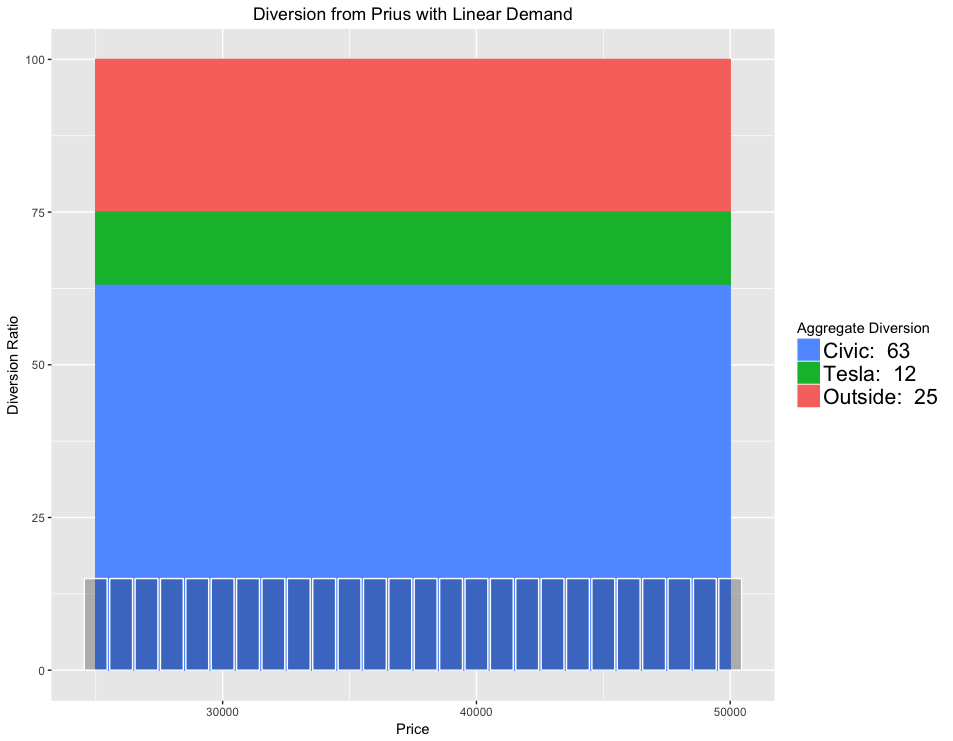
\includegraphics[width=4in]{./resources/new_prius_linear.png}
\end{center}
\end{frame}

\begin{frame}
\frametitle{Thought Experiment -- Inelastic CES Demand for a Prius}
\begin{center}
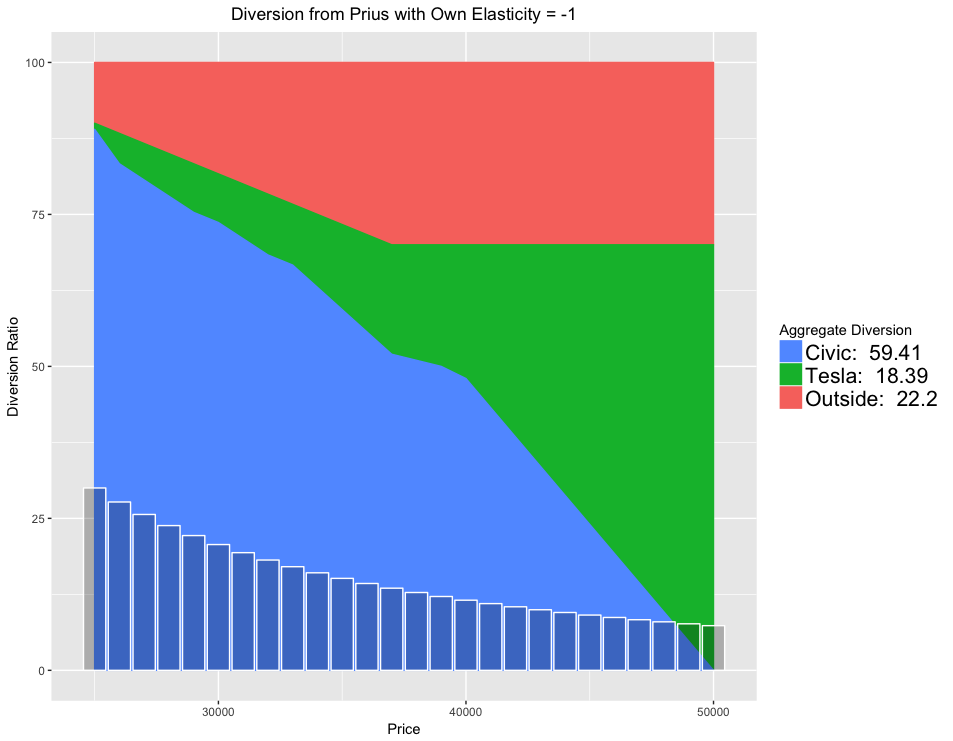
\includegraphics[width=4in]{./resources/new_prius1.png}
\end{center}
\end{frame}

\begin{frame}
\frametitle{Thought Experiment -- Elastic CES Demand for a Prius}
\begin{center}
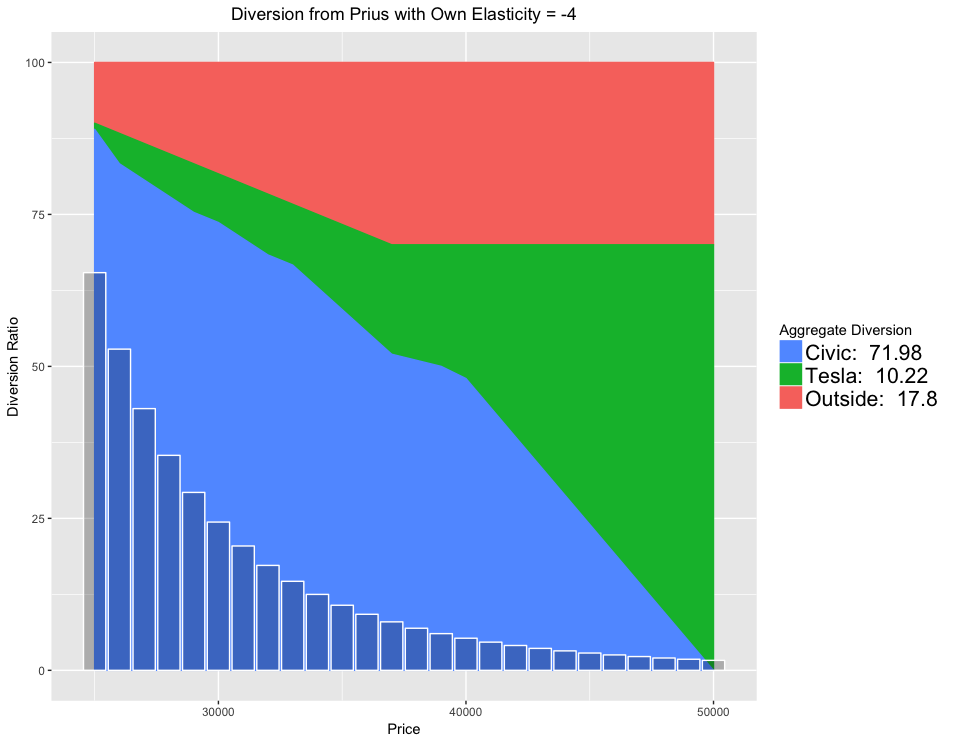
\includegraphics[width=4in]{./resources/new_prius4.png}
\end{center}
\end{frame}


\begin{frame}
\frametitle{Bias of Estimator}
\footnotesize
How far apart are $D_{jk}(\mathbf{p^0})$ and $\widehat{D_{jk}}$ when we increase price by $\Delta p_j$? 
\begin{eqnarray*}
\nonumber q_k(\mathbf{p}+ \Delta p_j) &\approx& q_k(\mathbf{p}) + \frac{\partial q_k}{\partial p_j} \Delta p_j + \frac{\partial^2 q_k}{\partial p_j^2} (\Delta p_j)^2 + O((\Delta p_j)^3) \\
\frac{ q_k(\mathbf{p}+ \Delta p_j)-q_k(\mathbf{p}) }{\Delta p_j} &\approx& \frac{\partial q_k}{\partial p_j}+ \frac{\partial^2 q_k}{\partial p_j^2} \Delta p_j + O(\Delta p_j)^2 \\
Bias(\widehat{D_{jk}} -D_{jk}(\mathbf{p^0})) &\approx& -  \frac{D_{jk} \frac{\partial^2 q_j}{\partial p_j^2} +  \frac{\partial^2 q_k}{\partial p_j^2} }{\frac{\partial q_j}{\partial p_j} + \frac{\partial^2 q_j}{\partial p_j^2}\Delta p_j } \Delta p_j
\end{eqnarray*}
\begin{itemize}
\item The downside of a large change $\Delta p_j$ is that the approximation of demand at $\mathbf{p^0}$ is less accurate and depends on the curvature of the demand function.
\item There are two demand models for which $Bias \equiv 0$ \alert{(constant treatment effects)}: \pause linear demand and plain IIA logit.
\end{itemize}
\end{frame}

\begin{frame}
\frametitle{Variance of Estimator}
\footnotesize
\begin{eqnarray*}
Var(\widehat{D_{jk} })&\approx& Var\left( \frac{\Delta q_k}{|\Delta q_j|} \right)\approx \frac{D_{jk} (1-D_{jk})}{\Delta q_j} \approx \frac{D_{jk} (1-D_{jk})}{\left| \frac{\partial q_j}{\partial p_j} \right| \Delta p_j}
\end{eqnarray*}
\normalsize
Variance is a problem when:
\begin{itemize}
\item  $\left| \frac{\partial q_j}{\partial p_j} \right| $ is small (inelastic demand $\rightarrow$ market power/ when we may be most worried about mergers).
\item $\Delta p_j \approx 0 $ (when price change is small).
\item Exacerbated by variation in $(q_j,q_k)$ unrelated to the exogenous price change (stochastic demand).
\end{itemize}
Bias-Variance tradeoff
\begin{itemize}
\item Precise measure of $\widehat{D_{jk}}^{ATE}$ or $\widehat{D_{jk}}^{LATE}$ for a large $\Delta p_j$ vs.
\item Noisy measure of $D_{jk}(\mathbf{p^0})$
\end{itemize}
\end{frame}


\begin{frame}
\footnotesize
\frametitle{Nevo (2000) and BLP (1999) Applications}
Data from Nevo (2000): $T=94$ markets, $J=24$ brands.
\begin{itemize}
\item RTE cereal (e.g., Kellogg's and General Mills merger)
\begin{eqnarray*}
u_{ijt} = d_{j} + x_{jt} \underbrace{(\overline{\beta} + \Sigma\cdot \nu_i + \Pi\cdot d_{it})}_{\beta_{it}} + \Delta \xi_{jt} + \varepsilon_{ijt}
\end{eqnarray*}

\begin{itemize}
\item[-] Features a large amount of preference heterogeneity, especially with respect to the price sensitivity $\beta_{it}^{price}$
\item[-] Estimated coefficient on price is distributed:
\begin{eqnarray*}
\scriptsize
\beta_{it}^{price} \sim N\left(\text{-63 + 588} \cdot \text{income}_{it} \text{ - 30} \cdot \text{inc}^2_{it}  \text{ + 11}\cdot \text{I[child]}_{it}, \sigma \text{=3.3}\right)
\end{eqnarray*}
\end{itemize}
\end{itemize}
%Because we have estimated a fully specified structural demand system, we can calculate the treatment effect measures easily:

Data from BLP (1999): $T=21$ markets, $J \approx 150$ products per market (total of 2271 product-market pairs)
\begin{itemize}
\item Random coefficients on vehicle size, miles-per-dollar, AC, horsepower/weight, constant. Price coefficient depends on income.
\end{itemize}
\end{frame}

%We denote a measure of diversion evaluated for an infinitessimally small price change as $MTE_p$, and a measure of diversion evaluated for an infinitessimally small change in quality as $MTE_q$. We refer to a `second choice' estimate of diversion as an ATE. For comparison, we also evaluated a Logit model, under which diversion is assumed to be constant. These four treatment effects are defined as:

\begin{frame}
\frametitle{Nevo (2000) and BLP (1999) Applications, cont.}
Define:

\begin{eqnarray*}
MTE = \frac{ \frac{\partial s_k}{\partial p_j}}{\left|\frac{\partial s_j}{\partial p_j}\right|},\quad  
%MTE_q =  \frac{ \frac{\partial s_k}{\partial \xi_j}}{ \left| \frac{\partial s_j}{\partial \xi_j} \right|},\quad 
ATE = \frac{s_k(A \setminus j) - s_k(A)}{\left| s_j(A \setminus j)- s_j(A ) \right|}, \quad
Logit = \frac{s_k(A)}{1-s_j(A)} 
\end{eqnarray*}
\begin{itemize}
\item Compare $MTE(\mathbf{p_0})$ to ATE
\item Compare $MTE(\mathbf{p_0})$ to Logit (Constant diversion, $\propto$ to share.)
\end{itemize}

%We suppose that the policy-relevant calculation of interest is the $MTE_p$, and we quantify how well the other treatment effect estimators approximate $MTE_p$. We compare $MTE_p$ to: $MTE_q$ (the marginal diversion ratio calculated by reducing the quality $\Delta \xi_{jt}$ of good $j$ rather than increasing its price); $ATE$ (the average treatment effect that we would identify from a product removal or second choice data); and $Logit$ (the diversion ratio we would estimate if we assumed that diversion was proportional to the marketshares as in the IIA logit model).

\end{frame}

\begin{frame}
\frametitle{Nevo (2000) Results}
Three Measures of Diversion
%\begin{table}[htp]
%\footnotesize
\begin{center}
\begin{tabular}{lrrr}
%\toprule
{} &  $MTE$  &  $ATE$ &  $Logit$  \\ \hline
%\midrule
%\midrule
& \multicolumn{3}{c}{Best Substitute}\\ \hline
%\midrule
Med($D_{jk}$)  &    13.26  &  13.54 &     9.05 \\
Mean($D_{jk}$) &    15.11  &  15.62 &    10.04 \\
\% Agree with MTE     &   &  89.98 &    58.38 \\ \hline
%\midrule
& \multicolumn{3}{c}{Outside Good}\\ \hline
%\midrule
Med($D_{j0}$)  &    35.30  &  32.40 &    54.43 \\
Mean($D_{j0}$) &    36.90 &  33.78 &    53.46 \\ \hline
%\bottomrule
\end{tabular}
\end{center}
%\caption{Substitution to Best Substitute and Outside Good}
%An observation is a product-market pair. There are 94 markets and 24 products.  
The first panel reports diversion to each product-market pair's best substitute. The second panel reports diversion to the outside good.
\end{frame}

\begin{frame}{BLP (1999) Results}
\begin{center}
\begin{tabular}{lrrr}
%\hline
{} &  $MTE$  &  $ATE$ &  $Logit$ \\ \hline
& \multicolumn{3}{c}{Best Substitute}\\ \hline
Med($D_{jk}$)  &    5.10 &   5.04 &   0.46 \\
Mean($D_{jk}$) &    6.07 &   6.25 &   0.53 \\
\% Agree with $MTE$    &  100.00 &  96.89 &  95.62 \\
\hline
& \multicolumn{3}{c}{Outside Good}\\ \hline
Med($D_{j0}$)  &   17.05 &  13.02 &  89.26 \\
Mean($D_{j0}$) &   17.04 &  13.44 &  89.36 \\ \hline
%\hline
\end{tabular}
\end{center}
The first panel reports diversion to each product-market pair's best substitute. The second panel reports diversion to the outside good.
\end{frame}

\begin{frame}
\frametitle{Nevo (2000) Results, cont.}

\% Difference in Diversion Measures: $y$ vs. $x=\log(\widehat{D^{MTE}(\mathbf{p_0}}))$
\begin{center}
\footnotesize
\begin{tabular}{l  rrrrr}
{} &  med($y-x$) &  mean($y-x$) &  med($|y-x|$) &  mean($|y-x|$) &  std($|y-x|$) \\ \hline
%\midrule
& \multicolumn{5}{c}{Best Substitutes}\\  \hline
%\midrule
%$MTE_q$ &        1.79 &         2.36 &          5.82 &           7.29 &          6.46 \\
$ATE$   &        2.56 &         3.24 &          6.00 &           7.61 &          7.04 \\
$Logit$ &      -44.19 &       -42.88 &         44.92 &          47.77 &         28.63 \\  \hline
%\midrule
& \multicolumn{5}{c}{All Products}\\  \hline
%\midrule
%$MTE_q$ &        5.65 &         8.40 &          8.17 &          12.14 &         12.27 \\
$ATE$   &        5.78 &         8.30 &          8.29 &          12.13 &         12.02 \\
$Logit$ &      -35.90 &       -25.92 &         49.48 &          53.27 &         34.56 \\  \hline
%\midrule
& \multicolumn{5}{c}{Outside Good}\\  \hline
%\midrule
%$MTE_q$ &       -7.46 &        -8.48 &          7.46 &           8.66 &          6.64 \\
$ATE$   &       -7.93 &        -8.89 &          7.94 &           9.08 &          6.77 \\
$Logit$ &       39.22 &        39.20 &         39.22 &          40.60 &         22.05 \\  \hline
%\bottomrule
\end{tabular}
%\caption{Relative \% Difference in Diversion Measures: Comparison $x=\log(\widehat{D^{MTE_p}})$}
%Notes: An observation is a product-market pair. There are 94 markets and 24 products.  
\end{center}

Table compares ATE and Logit measures of diversion to the MTE measure.

The first panel reports differences for each product-market pair's best substitute. 

The second panel averages across all possible substitutes. 

The third panel provides comparisons to the MTE diversion for the outside good.
%\label{tab:nevo2}

\end{frame}



\begin{frame}[plain]{BLP (1999) Results, cont.}
\% Difference in Diversion Measures: $y$ vs. $x=\log(\widehat{D^{MTE}(\mathbf{p_0}}))$

\begin{center}
\footnotesize
\begin{tabular}{l  rrrrr}
\toprule
{} &  med($y-x$) &  mean($y-x$) &  med($|y-x|$) &  mean($|y-x|$) &  std($|y-x|$) \\
& \multicolumn{5}{c}{Best Substitutes}\\ \midrule
$ATE$   &       -0.53 &         0.08 &         11.51 &          12.64 &          9.76 \\
$Logit$ &     -232.16 &      -239.75 &        232.16 &         239.75 &         40.58 \\ \hline
& \multicolumn{5}{c}{All Products}\\ \hline
$ATE$   &        9.79 &        26.52 &         22.54 &          40.34 &         47.85 \\
$Logit$ &     -183.79 &      -162.21 &        186.39 &         177.35 &         86.11 \\ \hline
& \multicolumn{5}{c}{Outside Good}\\ \hline
$ATE$   &      -23.62 &       -24.25 &         23.67 &          24.99 &         13.40 \\
$Logit$ &      165.42 &       186.43 &        165.42 &         186.43 &         72.86 \\ 
\bottomrule
\end{tabular}
\end{center}
\end{frame}


\begin{frame}
\frametitle{Lessons from Nevo (2000) and BLP (1999)}
\begin{itemize}
\item MTE vs. ATE measures are not hugely different in Nevo (2000).
\item Larger differences in BLP (1999). Why? More variation in quality, cost, and especially price -- better opportunity to observe larger differences in diversion.
\item ATE tends to predict slightly more inside substitution and less outside substitution. 
\item ATE may either overstate or understate diversion to other products on average. If the marginal consumer is more (less) inelastic as price increases, then ATE over- (under-) states diversion.
\item Both models rely on sum of diversion = 1.
\item Imposing proportional substitution (Logit) looks terrible.
\end{itemize}
\end{frame}


\begin{frame}{What's the point/Extensions}
\begin{itemize}
\item Calculating $D_{jk}$ or the matrix gives us the best idea about which products compete with each other.
\item What is wrong with cross-price elasticities?
\item Can we go from opportunity costs to prices?
\end{itemize}
\end{frame}



\section{Conduct}

\begin{frame}{Conduct Overview}
\begin{itemize}
\item A second set of important questions in IO is being able to use data to decide whether firms are \alert{competing} or \alert{colluding}.
\item Absent additional restrictions, we cannot generally look at data on $(P,Q)$ and decide whether or not collusion is taking place.
\item We can make progress in two ways: (1) parametric restrictions on marginal costs; (2) exclusion restrictions on supply.
\begin{itemize}
\item Most of the literature focuses on (1) by assuming something like: $\ln mc_{jt} = x_{jt} \gamma_1 + w_{jt} \gamma_2 + \omega_{jt}$.
\item In principle (2) is possible if we have instruments that shift demand for products but not supply. (These are much easier to come up with than ``supply shifters'').
\end{itemize}
\end{itemize}
\end{frame}

\begin{frame}{A famous plot (Bresnahan 87)}
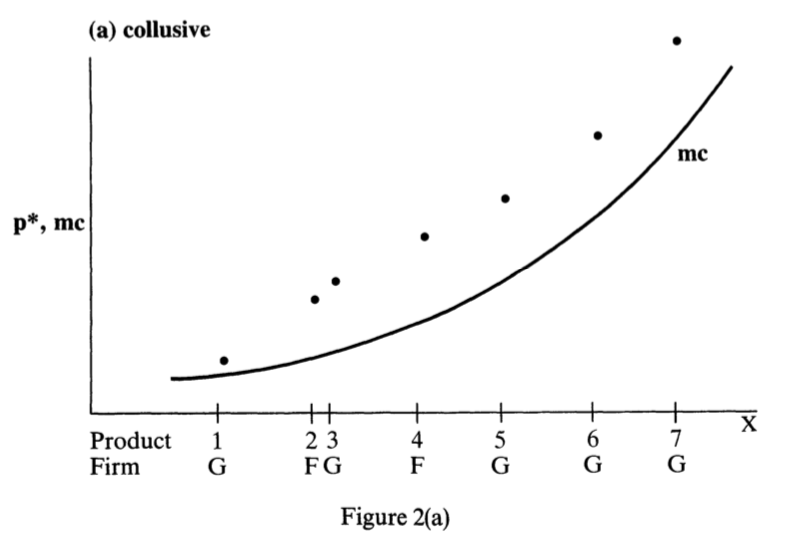
\includegraphics[width = 6.6cm]{./resources/bres_plot1.png}
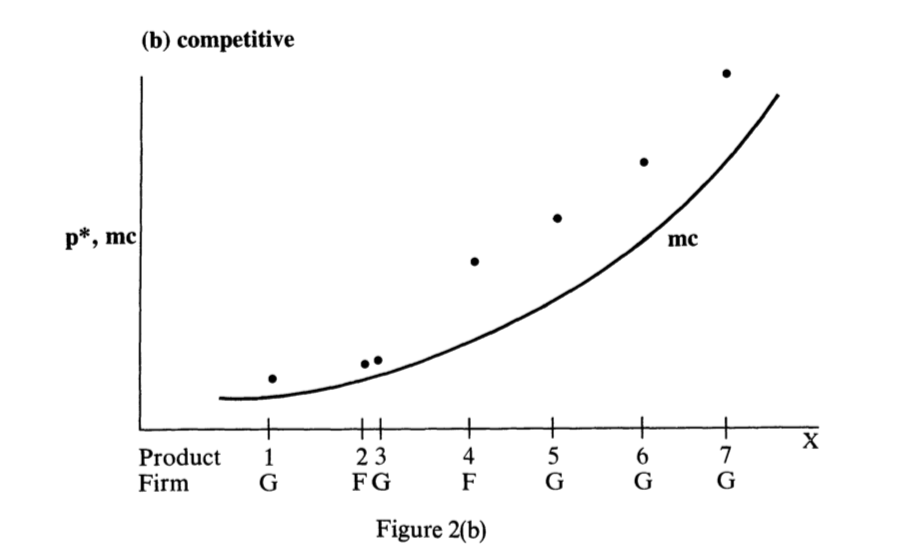
\includegraphics[width = 6.9cm]{./resources/bres_plot2.png}
\end{frame}



\begin{frame}{Testing For Conduct: Challenges}
\begin{itemize}
\item Recall the $\Omega$ matrix which we can write as $\Omega=\tilde{\Omega}\, \odot A$, where $\odot$ is the element-wise or Hadamard product of two matrices. 
\begin{itemize}
\item $\tilde{\Omega}$ is the matrix of demand derivatives with $\Omega_{(j,k)} = \frac{\partial q_j}{\partial p_k}$ for all elements.
\item $A_{(j,k)} =1$ if $(j,k)$ have the same owner and $0$ otherwise.
\end{itemize}
\item Mergers are about changing $0$'s to $1$'s in the $A$ matrix.
\item Matrix form of FOC: $q(\mathbf{p}) = \Omega(\mathbf{p})\cdot(\mathbf{p}-\mathbf{mc})$
\end{itemize}
\end{frame}

\begin{frame}
\frametitle{Testing For Collusion: Challenges}
We derived those conditions from multi-product Bertrand FOCs:
\begin{eqnarray*}
\arg \max_{p \in \mathcal{J}_f} \pi_f (\mathbf{p}) &=& \sum_{j \in \mathcal{J}_f} (p_j - c_j) \cdot q_j(\mathbf{p}) +  \alert{\kappa_{fg} \sum_{j \in \mathcal{J}_g} (p_j - c_j) \cdot q_j(\mathbf{p})} \\
\rightarrow 0&=& q_j(\mathbf{p}) + \sum_{k \in (\mathcal{J}_f,\mathcal{J}_g)} \alert{\kappa_{fg}}\cdot (p_k - c_k) \frac{\partial q_{k}}{\partial p_j}(\mathbf{p}) 
\end{eqnarray*}
\begin{itemize}
\item Now we have generalized the $A(\kappa)$ matrix.
\item Instead of $0$'s and $1$'s we now have $\kappa_{fg} \in [0,1]$ representing how much firm $f$ cares about the profits of $g$.
\begin{itemize}
\item If $f$ and $g$ merge (or fully colluded) then $\kappa_{fg} =1$
\item Often in the real world firms cannot reach fully collusive profits and $\kappa_{fg} \in (0,1)$.
\item Evidence that $\kappa_{fg} > 0$ is not necessarily evidence of malfeasance, just a deviation from \alert{static Bertrand pricing}.
\end{itemize}
\end{itemize}
\end{frame}

\begin{frame}
\frametitle{Reasons for Deviations from Static Bertrand}
\small
\begin{description}
\item[Biased estimates of own and cross price derivatives:] For anything to work, you have correct estimates of $\tilde{\Omega}$. My prior is most papers \alert{underestimate} cross price elasticites.
\item[Vertical Relationships:] Who sets supermarket prices? Just the retailer? Just the manufacturer? Some combination of both? Retailers tend to \alert{soften} downstream price competition.
\item[Faulty Timing Assumptions:] Bertrand is a simultaneous move pricing game. Lots of alternatives (Stackelberg leader-follower, Edgeworth cycles, etc.).
\item[Dynamics and Dynamic Pricing:] Forward looking firms or consumers might not set static Nash prices. [e.g. Temporary Sales, Switching Costs, Network Effects, etc.]
\item[Unmodeled Supergame:] Maybe firms are legally tacitly colluding, higher prices might be about what firms believe will happen in a price war.
\end{description}
\end{frame}



\begin{frame}
\frametitle{Algorithm \#1: Bertrand Deviations}

\begin{itemize}
\item Recover $\tilde{\Omega}$ from demand alone.
\item Recover marginal costs $\widehat{\mathbf{mc}} = \mathbf{p} +(O.*\tilde{\Omega}(\mathbf{p}))^{-1} q(\mathbf{p})$.
\end{itemize}
Challenges:
\begin{itemize}
\item Given $[\mathbf{q},\mathbf{p},\tilde{\Omega},O]$ I can always produce a vector of marginal costs $\mathbf{c}$ that rationalizes what we observe. [ie: $J$ equations $J$ unknowns].
\item Maybe some vectors of $\mathbf{c}$ look less ``reasonable'' than others.
\begin{itemize}
\item ie: I have a parametric model of MC in mind. 
\item Can test that model with GMM objective of $c_{jt}$ on regressors.
\item Maybe marginal costs cannot deviate too much within product from period to period.
\item Marginal costs $\leq 0$ seem problematic. [Might just be that your estimates for demand are too inelastic...]
\end{itemize}
\end{itemize}
\end{frame}

\begin{frame}
\frametitle{Algorithm \#2: Simultaneous Supply and Demand}
\begin{itemize}
\item Recover $\tilde{\Omega}$ from demand and parametric assumption on supply (GMM with both sets of moments).
\item I can impose $c > 0$ by using $\ln mc_{jt} = x_{jt} \gamma_1 + w_{jt} \gamma_2 + \omega_{jt}$.
\item The fit of my supply side will also inform my demand parameters, particularly $\alpha$ the price coefficient. [BLP 95 used this for additional power with lots of random coefficients and potentially weak instruments].
\end{itemize}
Challenges:
\begin{itemize}
\item Am I testing conduct? Or am I testing the linear functional form for my supply model?
\item Will a missing $z_{jt}$ change whether or not I believe firms are colluding?
\end{itemize}
\end{frame}



\begin{frame}{\normalsize Algorithm \#3: Exclusion Restrictions}
\small
\begin{itemize}
\item We provide a formal test for four alternative models of conduct based on the exclusion restriction test in Berry and Haile (2014) 
\begin{eqnarray*}
\widehat{mc_{jt}}(\kappa,\hat{\theta}) &=& \lambda_j +  \gamma_1 x_{jt} + \gamma_2 w_{jt} + \omega_{jt}\\
\omega_{jt} &=& \widehat{mc_{jt}}(\kappa,\hat{\theta}) - \lambda_j -  \gamma_1 x_{jt} - \gamma_2 w_{jt} \\
0 &=& E[ \omega_{jt} | \lambda_j, x_{jt}, w_{jt}, \alert{z_{jt}^s}]
\end{eqnarray*}
\item $w_{jt}$: cost shifters (price of corn for Corn Flakes, price of rice for Rice Krispies).
\item $z_{jt}^s$: should \alert{not} shift marginal costs under the true model of conduct but could potentially shift marginal costs under the alternative. A good choice is \alert{markup shifters}.
\begin{itemize}
\item BLP instruments
\item Cost shifters for other products (Price of Rice for Corn Flakes, Price of Corn for Rice Krispies).
\item $\kappa$ parameters or $\kappa$ weighted diversion.
\end{itemize}
\end{itemize}
\end{frame}

\begin{frame}{Start with BLP(95/99) / Nevo (2001)}
Utility of consumer $i$ for product $j$ and store-week $t$ as:
\begin{align*}
    u_{ijt} = \delta_{jt}+ \mu_{ijt}+  \epsilon_{ijt}
\end{align*}
Market shares are given by:
\begin{align*}
    s_{jt}(\delta_{\cdot t},\theta_2) = \int \frac{\exp[ \delta_{jt} + \mu_{ijt} ]}{\sum_{k \in J_t} \exp[ \delta_{kt} + \mu_{ikt} ]} f(\mu_{it} \mid \widetilde{\theta}_2) \, d\mu_{it}.
\end{align*}
BH2014 show that one can invert the vector of observed market shares $\mathcal{S}_t$ to solve for $\delta_{t}=D_{t}^{-1}(\mathcal{S}_t, \theta_2)$.\\
\end{frame}

\begin{frame}[plain]
\frametitle{Supply Side}
Consider the multi-product Bertrand FOCs:
\footnotesize
{\begin{eqnarray*}
\arg \max_{p \in \mathcal{J}_f} \pi_f (\mathbf{p}) &=& \sum_{j \in \mathcal{J}_f} (p_j - c_j) \cdot s_j(\mathbf{p}) +  \kappa_{fg}\sum_{k \in \mathcal{J}_g} (p_k - c_k) \cdot s_k(\mathbf{p}) \\
0&=& s_j(\mathbf{p}) + \sum_{k \in \mathcal{J}_f} (p_k - c_k) \frac{\partial s_{k}}{\partial p_j}(\mathbf{p}) + \sum_g  \alert{\kappa_{fg} \sum_{l \in \mathcal{J}_g} (p_l - c_l) \frac{\partial s_{l}}{\partial p_j}(\mathbf{p})}\\
\end{eqnarray*}
}
It is helpful to define the matrix $\Omega_{(j,k)}(\mathbf{p})  = - \frac{\partial s_{j}}{\partial p_k}(\mathbf{p})$:
\begin{eqnarray*}
A(\kappa)_{(j,k)} = \left\{\begin{array}{lr}
          1 & \text{for }  j \in \mathcal{J}_f \\ 
       	  \kappa_{fg} & \text{for }  j \in \mathcal{J}_f, k \in \mathcal{J}_g\\
	  0 & \text{o.w}\\
        \end{array} \right\}
\end{eqnarray*}
We can re-write the FOC in matrix form:
\begin{eqnarray*}
        s(\mathbf{p}) &= (A(\kappa) \odot \Omega(\mathbf{p})) \cdot (\mathbf{p} - \mathbf{mc}), \\
       \mathbf{mc} &=  \mathbf{p} - \underbrace{(A(\kappa) \odot \Omega(\mathbf{p}))^{-1} s(\mathbf{p})}_{\eta(\mathbf{p},\mathbf{s},\theta_2,\kappa)}.
\end{eqnarray*}
\end{frame}

\begin{frame}{Simultaneous Problem}
Assume additivity, and write in terms of structural errors:
\begin{align*}
\xi_{jt} &=\delta_{jt}(\mathcal{S}_t,\widetilde{\theta}_2) - \theta_1[x_{jt}, \, \alert{v_{jt}}] - \alpha p_{jt} \\
\omega_{jt} &= f \left( p_{jt} - \eta_{jt}(\mathbf{p},\mathbf{s},\theta_2,\kappa) \right) - h(x_{jt}, \alert{w_{jt}},\theta_3)
\end{align*}
We've highlighted the two \alert{exclusion restrictions}:
\begin{itemize}
\item Cost shifters $w_{jt}$
\item Demand shifters $v_{jt}$
\end{itemize}
To simplify slides we let $f(x)=x$ (often $f(x) =\log(x))$.
\end{frame}

\begin{frame}{Simultaneous Problem: Menu Approach}
Assume two models of conduct (correct: $\kappa_0$) (incorrect: $\kappa_1$)
\begin{align*}
%\label{eq:both_mc}
f(p_{jt} -\eta_{jt}(\kappa_0))= h(x_{jt},w_{jt};\theta_3^0)+  \omega_{jt}^{0},\\
f(p_{jt} -\eta_{jt}(\kappa_1))= h(x_{jt},w_{jt};\theta_3^1)+  \omega_{jt}^{1}.
\end{align*}
Write things in terms of the markup difference:
\begin{align*}
p_{jt} -\eta_{jt}(\kappa_1)= h(x_{jt},w_{jt};\theta_3)+ \overbrace{\lambda \cdot  \Delta \eta_{jt}(\mathbf{p},\mathbf{s},\theta,\kappa_0,\kappa_1) +   \omega_{jt}}^{\widetilde{\omega_{jt}}}
\end{align*}
Tempting idea: run the above regression and test if $\lambda=0$.
\begin{itemize}
\item True model $\lambda=0$, alternate model $\lambda \neq 0$. \pause
\item $\eta_{jt}$ is \alert{endogenous}: it depends on everything including $(\xi,\omega)$.
\end{itemize}
\end{frame}


\begin{frame}{An Old Problem}
\begin{itemize}
\item Bresnahan (1980/1982) recognized this problem: we need ``rotations of demand''.
\item Most of the literature followed Bresnahan (1987):
\begin{itemize}
\item $\omega_{jt}$ is \alert{measurement error in price} 
\item Ex: Bonnet and Dubois (2010) $E[\ln(\omega_{jt}) | x_{jt},w_{jt}]=0$:
\begin{align*}
\log(p_{jt} -\eta_{jt}(\kappa,\widehat{\theta}_2))) = h(x_{jt},w_{jt},\theta_3) + \ln \omega_{jt}
\end{align*}
\end{itemize}
\item Other idea: put markup back on RHS and test $\lambda=1$
\begin{align*}
p_{jt} = h(x_{jt},w_{jt},\theta_3)+ \lambda\cdot  \eta_{jt}(\kappa,\widehat{\theta}_2)+ \omega_{jt}
\end{align*}
\begin{itemize}
\item ``Informal'' test of Villas Boas (2007): $E[\omega_{jt} | x_{jt},w_{jt}]=0$.
\item Pakes (2017) uses Wollman (2018) data and BLP IV $E[\omega_{jt} | x_{jt},w_{jt},f(x_{-j})]=0$.
\end{itemize}
\end{itemize}
\end{frame}

\begin{frame}{A subtle solution}
\begin{itemize}
\item Berry Haile 2014 tell us we need \alert{marginal revenue shifters} to act as \alert{exclusion restrictions}.
\item We need an instrument for $\Delta \eta_{jt}(\mathbf{p},\mathbf{s},\theta,\kappa_0,\kappa_1)$
\begin{itemize}
\item Maybe not so hard since it is basically a function of everything.
\item Cannot have a direct effect on $mc_{jt}$ (exclusion restriction).
\end{itemize}
\item Idea would be to use $E[\omega_{jt} | x_{jt}, w_{jt}, z_{jt}^S]=0$:
\begin{align*}
 p_{jt} - \eta_{jt}(\mathbf{p},\mathbf{s},\theta_2,\kappa)  =  h(x_{jt}, w_{jt},\theta_3)  + \omega_{jt} 
\end{align*}
\end{itemize}
\end{frame}

\begin{frame}{Candidate Instruments for $z_{jt}^s$}
\begin{enumerate}
\item The demand shifter $v_{jt}$: maybe easy to find??
\begin{itemize}
\item We use product recalls; prices of complements don't work so well.
\end{itemize}
\item BLP instruments $f(x_{-j})$: not always strong
\begin{itemize}
\item Amit and JF have a nice paper showing how to choose $f(x_{-j})$
\end{itemize}
\item Can use the same logic to construct $v_{-jt}$ or $w_{-jt}$
\begin{itemize}
\item ie: cost shifters (or demand shifters) of competing goods.
\item Price of rice for Corn Flakes; price of corn for Rice Krispies.
\item Will depend on closeness of substitutes $\Delta PPI$ or $D_{jk}$.
\end{itemize}
\item Observed Conduct Shifters: $\kappa_{fg}$
\begin{itemize}
\item Usually conduct is \alert{unobserved} if we are testing it!
\item Index Inclusion Events (Fiona, Kennedy et. al); BlackRock-BGI Acquisition (AST)
\item Miller Weinberg (2017) use (pre/post merger for cartel participants).
\end{itemize}
\end{enumerate}
\end{frame}

\begin{frame}{Things that don't work}
\begin{itemize}
\item $\xi_{jt}$ only makes sense if you believe $Cov(\xi_{jt},\omega_{jt})=0$.
\item $p_{j,t,-s}$ (Hausman instruments) same good in other markets: pick up cost shocks (but could pick up changes in conduct!). 
\item If it isn't in one of our equations: does it have anything to do with demand or supply?
\item It turns out that 2SLS analog $E[\Delta \eta_{jt} | x_t, w_t, v_t,Z_{jt}^e]=\widehat{\Delta \eta_{jt}}$ doesn't add much:
\begin{itemize}
\item Markups aren't a linear function of observables.
\item Coefficients are (probably) quite different across products.
\end{itemize}
\end{itemize}
\end{frame}













\end{document}